\documentclass[]{article}
\usepackage{lmodern}
\usepackage{amssymb,amsmath}
\usepackage{ifxetex,ifluatex}
\usepackage{fixltx2e} % provides \textsubscript
\ifnum 0\ifxetex 1\fi\ifluatex 1\fi=0 % if pdftex
  \usepackage[T1]{fontenc}
  \usepackage[utf8]{inputenc}
\else % if luatex or xelatex
  \ifxetex
    \usepackage{mathspec}
  \else
    \usepackage{fontspec}
  \fi
  \defaultfontfeatures{Ligatures=TeX,Scale=MatchLowercase}
\fi
% use upquote if available, for straight quotes in verbatim environments
\IfFileExists{upquote.sty}{\usepackage{upquote}}{}
% use microtype if available
\IfFileExists{microtype.sty}{%
\usepackage{microtype}
\UseMicrotypeSet[protrusion]{basicmath} % disable protrusion for tt fonts
}{}
\usepackage[margin=1in]{geometry}
\usepackage{hyperref}
\PassOptionsToPackage{usenames,dvipsnames}{color} % color is loaded by hyperref
\hypersetup{unicode=true,
            pdftitle={Session regression I: simple linear regression},
            colorlinks=true,
            linkcolor=Maroon,
            citecolor=Blue,
            urlcolor=blue,
            breaklinks=true}
\urlstyle{same}  % don't use monospace font for urls
\usepackage{color}
\usepackage{fancyvrb}
\newcommand{\VerbBar}{|}
\newcommand{\VERB}{\Verb[commandchars=\\\{\}]}
\DefineVerbatimEnvironment{Highlighting}{Verbatim}{commandchars=\\\{\}}
% Add ',fontsize=\small' for more characters per line
\usepackage{framed}
\definecolor{shadecolor}{RGB}{248,248,248}
\newenvironment{Shaded}{\begin{snugshade}}{\end{snugshade}}
\newcommand{\AlertTok}[1]{\textcolor[rgb]{0.94,0.16,0.16}{#1}}
\newcommand{\AnnotationTok}[1]{\textcolor[rgb]{0.56,0.35,0.01}{\textbf{\textit{#1}}}}
\newcommand{\AttributeTok}[1]{\textcolor[rgb]{0.77,0.63,0.00}{#1}}
\newcommand{\BaseNTok}[1]{\textcolor[rgb]{0.00,0.00,0.81}{#1}}
\newcommand{\BuiltInTok}[1]{#1}
\newcommand{\CharTok}[1]{\textcolor[rgb]{0.31,0.60,0.02}{#1}}
\newcommand{\CommentTok}[1]{\textcolor[rgb]{0.56,0.35,0.01}{\textit{#1}}}
\newcommand{\CommentVarTok}[1]{\textcolor[rgb]{0.56,0.35,0.01}{\textbf{\textit{#1}}}}
\newcommand{\ConstantTok}[1]{\textcolor[rgb]{0.00,0.00,0.00}{#1}}
\newcommand{\ControlFlowTok}[1]{\textcolor[rgb]{0.13,0.29,0.53}{\textbf{#1}}}
\newcommand{\DataTypeTok}[1]{\textcolor[rgb]{0.13,0.29,0.53}{#1}}
\newcommand{\DecValTok}[1]{\textcolor[rgb]{0.00,0.00,0.81}{#1}}
\newcommand{\DocumentationTok}[1]{\textcolor[rgb]{0.56,0.35,0.01}{\textbf{\textit{#1}}}}
\newcommand{\ErrorTok}[1]{\textcolor[rgb]{0.64,0.00,0.00}{\textbf{#1}}}
\newcommand{\ExtensionTok}[1]{#1}
\newcommand{\FloatTok}[1]{\textcolor[rgb]{0.00,0.00,0.81}{#1}}
\newcommand{\FunctionTok}[1]{\textcolor[rgb]{0.00,0.00,0.00}{#1}}
\newcommand{\ImportTok}[1]{#1}
\newcommand{\InformationTok}[1]{\textcolor[rgb]{0.56,0.35,0.01}{\textbf{\textit{#1}}}}
\newcommand{\KeywordTok}[1]{\textcolor[rgb]{0.13,0.29,0.53}{\textbf{#1}}}
\newcommand{\NormalTok}[1]{#1}
\newcommand{\OperatorTok}[1]{\textcolor[rgb]{0.81,0.36,0.00}{\textbf{#1}}}
\newcommand{\OtherTok}[1]{\textcolor[rgb]{0.56,0.35,0.01}{#1}}
\newcommand{\PreprocessorTok}[1]{\textcolor[rgb]{0.56,0.35,0.01}{\textit{#1}}}
\newcommand{\RegionMarkerTok}[1]{#1}
\newcommand{\SpecialCharTok}[1]{\textcolor[rgb]{0.00,0.00,0.00}{#1}}
\newcommand{\SpecialStringTok}[1]{\textcolor[rgb]{0.31,0.60,0.02}{#1}}
\newcommand{\StringTok}[1]{\textcolor[rgb]{0.31,0.60,0.02}{#1}}
\newcommand{\VariableTok}[1]{\textcolor[rgb]{0.00,0.00,0.00}{#1}}
\newcommand{\VerbatimStringTok}[1]{\textcolor[rgb]{0.31,0.60,0.02}{#1}}
\newcommand{\WarningTok}[1]{\textcolor[rgb]{0.56,0.35,0.01}{\textbf{\textit{#1}}}}
\usepackage{graphicx,grffile}
\makeatletter
\def\maxwidth{\ifdim\Gin@nat@width>\linewidth\linewidth\else\Gin@nat@width\fi}
\def\maxheight{\ifdim\Gin@nat@height>\textheight\textheight\else\Gin@nat@height\fi}
\makeatother
% Scale images if necessary, so that they will not overflow the page
% margins by default, and it is still possible to overwrite the defaults
% using explicit options in \includegraphics[width, height, ...]{}
\setkeys{Gin}{width=\maxwidth,height=\maxheight,keepaspectratio}
\IfFileExists{parskip.sty}{%
\usepackage{parskip}
}{% else
\setlength{\parindent}{0pt}
\setlength{\parskip}{6pt plus 2pt minus 1pt}
}
\setlength{\emergencystretch}{3em}  % prevent overfull lines
\providecommand{\tightlist}{%
  \setlength{\itemsep}{0pt}\setlength{\parskip}{0pt}}
\setcounter{secnumdepth}{0}
% Redefines (sub)paragraphs to behave more like sections
\ifx\paragraph\undefined\else
\let\oldparagraph\paragraph
\renewcommand{\paragraph}[1]{\oldparagraph{#1}\mbox{}}
\fi
\ifx\subparagraph\undefined\else
\let\oldsubparagraph\subparagraph
\renewcommand{\subparagraph}[1]{\oldsubparagraph{#1}\mbox{}}
\fi

%%% Use protect on footnotes to avoid problems with footnotes in titles
\let\rmarkdownfootnote\footnote%
\def\footnote{\protect\rmarkdownfootnote}

%%% Change title format to be more compact
\usepackage{titling}

% Create subtitle command for use in maketitle
\newcommand{\subtitle}[1]{
  \posttitle{
    \begin{center}\large#1\end{center}
    }
}

\setlength{\droptitle}{-2em}

  \title{Session regression I: simple linear regression}
    \pretitle{\vspace{\droptitle}\centering\huge}
  \posttitle{\par}
    \author{}
    \preauthor{}\postauthor{}
    \date{}
    \predate{}\postdate{}
  
\usepackage{float}

\begin{document}
\maketitle

\hypertarget{learning-outcomes}{%
\subsection{Learning outcomes}\label{learning-outcomes}}

\begin{itemize}
\tightlist
\item
  understand simple linear regression model incl.~terminology and
  mathematical notations
\item
  estimate model parameters and their standar error
\item
  use model for checking the association between \emph{x} and \emph{y}
\item
  use model for prediction
\item
  assees model accuracy with RSE and R\(^2\)
\item
  check model assumptions
\item
  to be able to use \texttt{lm} function in R for model fitting,
  obtaining confidence interval and predictions
\end{itemize}

\begin{center}\rule{0.5\linewidth}{\linethickness}\end{center}

\hypertarget{introduction}{%
\subsection{Introduction}\label{introduction}}

\begin{itemize}
\tightlist
\item
  \href{https://forms.gle/bHZr1MP454npysAFA}{Quiz}: What do we already
  know about \texttt{simple\ linear\ regression}?
\end{itemize}

\hypertarget{description}{%
\paragraph{Description}\label{description}}

\begin{itemize}
\tightlist
\item
  Simple linear regression is a statistical method that allows us to
  summarize and study relationships between two continuous
  (quantitative, numerical) variables

  \begin{itemize}
  \tightlist
  \item
    one variable, denoted \texttt{x} is regarded as the
    \emph{predictor}, \emph{explanatory}, or \emph{indepedent variable},
    e.g.~body weight (kg)
  \item
    the other variable, denoted \texttt{y}, is regarded as the
    \emph{response}, \emph{outcome}, or \emph{dependent variable},
    e.g.~plasma volume (l)
  \end{itemize}
\item
  It is used to estimate the best-fitting straight line to describe the
  association
\end{itemize}

\hypertarget{used-for-to-answer-questions-such-as}{%
\paragraph{Used for to answer questions such
as:}\label{used-for-to-answer-questions-such-as}}

\begin{itemize}
\tightlist
\item
  is there a relationship between \texttt{x} exposure (e.g.~body weight)
  and \texttt{y} outcome (e.g.~plasma volume)?
\item
  how strong is the relationship between the two variables?
\item
  what will be a predicted value of the \texttt{y} outcome given a new
  set of exposure values?
\item
  how accurately can we predict the outcome?
\end{itemize}

\newpage

\begin{figure}
\centering
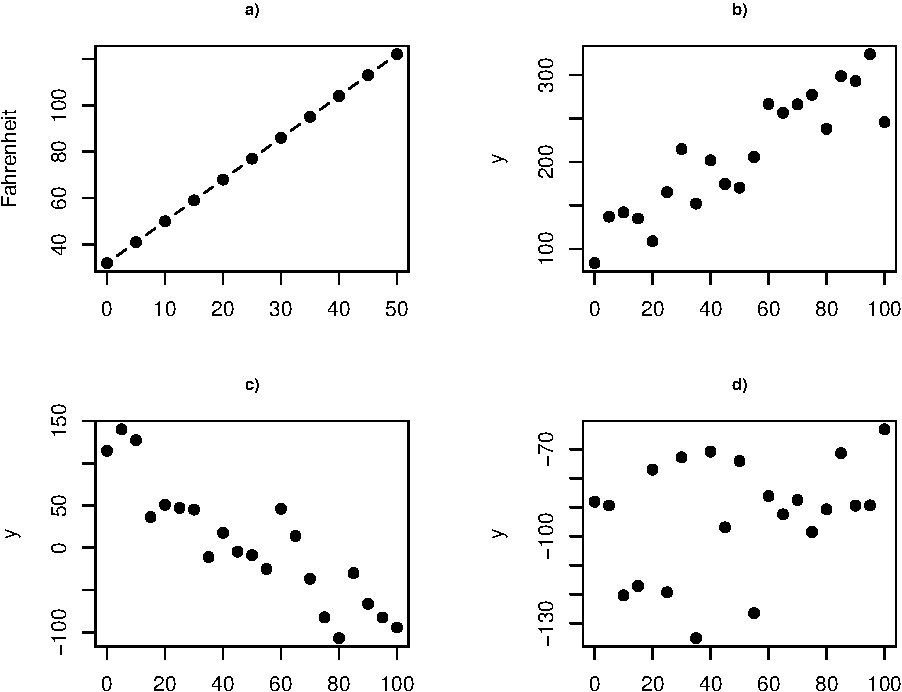
\includegraphics{session-regression-I-files/figures/det-vs-stat-1.pdf}
\caption{\textbf{Determinisitc vs.~statistical relationship}: a)
deterministic: equation exactly describes the relationship between the
two variables e.g.~\(Fahrenheit=9/5*Celcius+32\); b) statistical
relationship between x and y is not perfect (increasing), c) statistical
relationship between x and y is not perfect (decreasing), d) random
signal}
\end{figure}

\hypertarget{example-data}{%
\subsubsection{Example data}\label{example-data}}

Example data contain the body weight and plasma volume for eight healthy
men.

\begin{Shaded}
\begin{Highlighting}[]
\NormalTok{weight <-}\StringTok{ }\KeywordTok{c}\NormalTok{(}\DecValTok{58}\NormalTok{, }\DecValTok{70}\NormalTok{, }\DecValTok{74}\NormalTok{, }\FloatTok{63.5}\NormalTok{, }\FloatTok{62.0}\NormalTok{, }\FloatTok{70.5}\NormalTok{, }\FloatTok{71.0}\NormalTok{, }\FloatTok{66.0}\NormalTok{) }\CommentTok{# body weight (kg)}
\NormalTok{plasma <-}\StringTok{ }\KeywordTok{c}\NormalTok{(}\FloatTok{2.75}\NormalTok{, }\FloatTok{2.86}\NormalTok{, }\FloatTok{3.37}\NormalTok{, }\FloatTok{2.76}\NormalTok{, }\FloatTok{2.62}\NormalTok{, }\FloatTok{3.49}\NormalTok{, }\FloatTok{3.05}\NormalTok{, }\FloatTok{3.12}\NormalTok{) }\CommentTok{# plasma volume (liters)}
\end{Highlighting}
\end{Shaded}

Scatter plot of the data shows that high plasma volume tends to be
associated with high weight and \emph{vice verca}. Linear regrssion
gives the equation of the straight line that best describes how the
outcome changes (increase or decreases) with a change of exposure
variable (in red)

\begin{center}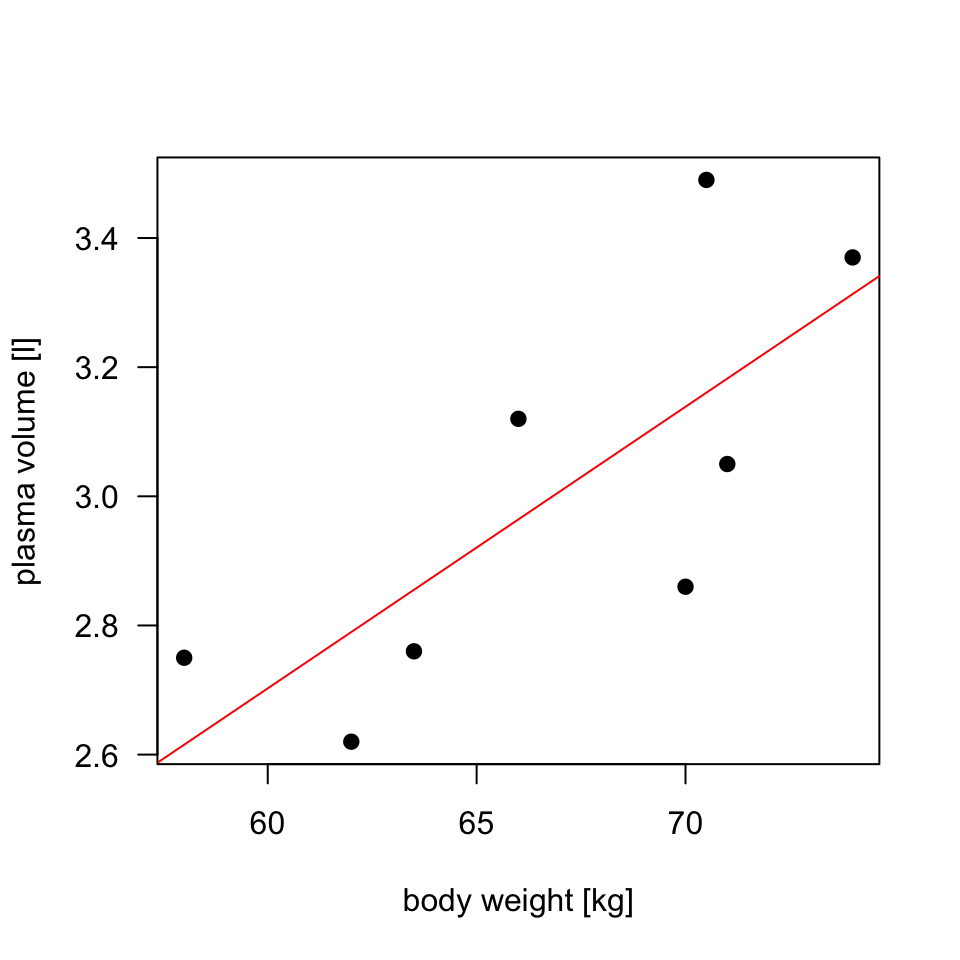
\includegraphics{session-regression-I-files/figures/fig-reg-1} \end{center}

The equation of the regression line is:

\[y=beta_0 + beta_1x\]

\hypertarget{estimating-the-coefficients}{%
\subsubsection{Estimating the
Coefficients}\label{estimating-the-coefficients}}

\hypertarget{assessing-the-accuracy-of-the-coefficient-estimates}{%
\subsubsection{Assessing the Accuracy of the Coefficient
Estimates}\label{assessing-the-accuracy-of-the-coefficient-estimates}}

\hypertarget{asesssing-the-accuracy-of-the-model}{%
\subsubsection{Asesssing the Accuracy of the
Model}\label{asesssing-the-accuracy-of-the-model}}

\begin{verbatim}
## [1] 0.7591266
\end{verbatim}

\begin{verbatim}
## 
## Call:
## lm(formula = y ~ x)
## 
## Residuals:
##      Min       1Q   Median       3Q      Max 
## -0.27880 -0.14178 -0.01928  0.13986  0.32939 
## 
## Coefficients:
##             Estimate Std. Error t value Pr(>|t|)  
## (Intercept)  0.08572    1.02400   0.084   0.9360  
## x            0.04362    0.01527   2.857   0.0289 *
## ---
## Signif. codes:  0 '***' 0.001 '**' 0.01 '*' 0.05 '.' 0.1 ' ' 1
## 
## Residual standard error: 0.2188 on 6 degrees of freedom
## Multiple R-squared:  0.5763, Adjusted R-squared:  0.5057 
## F-statistic:  8.16 on 1 and 6 DF,  p-value: 0.02893
\end{verbatim}

\begin{verbatim}
##          x 
## 0.01526836
\end{verbatim}

\begin{verbatim}
##        x 
## 1.023998
\end{verbatim}

\hypertarget{multiple-linear-regression}{%
\subsection{Multiple linear
regression}\label{multiple-linear-regression}}

\hypertarget{estimating-the-regression-coefficients}{%
\subsubsection{Estimating the Regression
Coefficients}\label{estimating-the-regression-coefficients}}

\hypertarget{estimating-coefficients}{%
\subsubsection{Estimating coefficients}\label{estimating-coefficients}}

\hypertarget{relationship-between-the-response-and-predictors}{%
\subsubsection{Relationship between the response and
predictors}\label{relationship-between-the-response-and-predictors}}

\hypertarget{model-fit}{%
\subsubsection{Model fit}\label{model-fit}}

\hypertarget{predictions}{%
\subsubsection{Predictions}\label{predictions}}

\hypertarget{qualitative-predictors}{%
\subsubsection{Qualitative predictors}\label{qualitative-predictors}}

\hypertarget{interaction-terms}{%
\subsubsection{Interaction terms}\label{interaction-terms}}

\hypertarget{non-linear-transformation-of-the-predictors}{%
\subsubsection{Non-linear transformation of the
predictors}\label{non-linear-transformation-of-the-predictors}}

\hypertarget{potential-problems-non-linearity-collinearity}{%
\subsubsection{Potential problems: non-linearity,
collinearity}\label{potential-problems-non-linearity-collinearity}}

\hypertarget{logistic-regression}{%
\subsubsection{Logistic regression}\label{logistic-regression}}


\end{document}
